\section{Experimental Evaluation}
\label{sec:experiments}

Most of the traffic in our data center is intra-DC traffic: VMs communicating
with VMs in the same DC. We emulate this scenario using two Dell PowerEdge R410
servers.  Both servers have four 2.26GHz cores, with hyper-threading enabled,
which gives it 8 logical processors.  Each machine has 8GB of RAM and 10G NIC.
Both machines run a flavor of Windows Server OS with Hyper-V enabled for network
virtualization. 

Given the lack of space, we only present limited results in this section,
focusing mostly on microbenchmarks. Our primary goal is to demonstrate that the
values we selected for the three important parameters, viz:

\subsection{Picking a Timer Period for Measurement}

{\bf Question:}  What value of $T$ should we pick for the algorithm. Recall $T$
is the time between macroscheduler invocations.

{\bf Motivation:}  The frequency of the macroscheduler adjusting the allocated
rates determins how quicklya  customer VM can cahieve its minimum guranteed
bandwidth.  As shown earlier, it can take up to 4 iterations (thus $4*T$ time
units) for the macro-scheduler to allocate a VM with its minimum guaranteed
bandwidth. So we don't want $T$ to be too large. On the other hand, if $T$ is
too small, the measured send rate of the VM ($SR$) may be inaccurate. 

{\bf Experiment}: We have a single VM send data as fast as possible, using
several TCP connections. The VM's bandwidth was limited to 7.2Gbps using the
rate limiter, and all other rate allocation functionality was disabled.  We
logged the measured send rate ($SR$) over 100 intervals.  We repeat the
experiment with varying the iteration time from 15ms to 1000ms, and compute the
percent standard deviation for each value of $T$. 

Figure~\ref{variation} shows the effect of different interval times.  

\begin{figure}
\centering
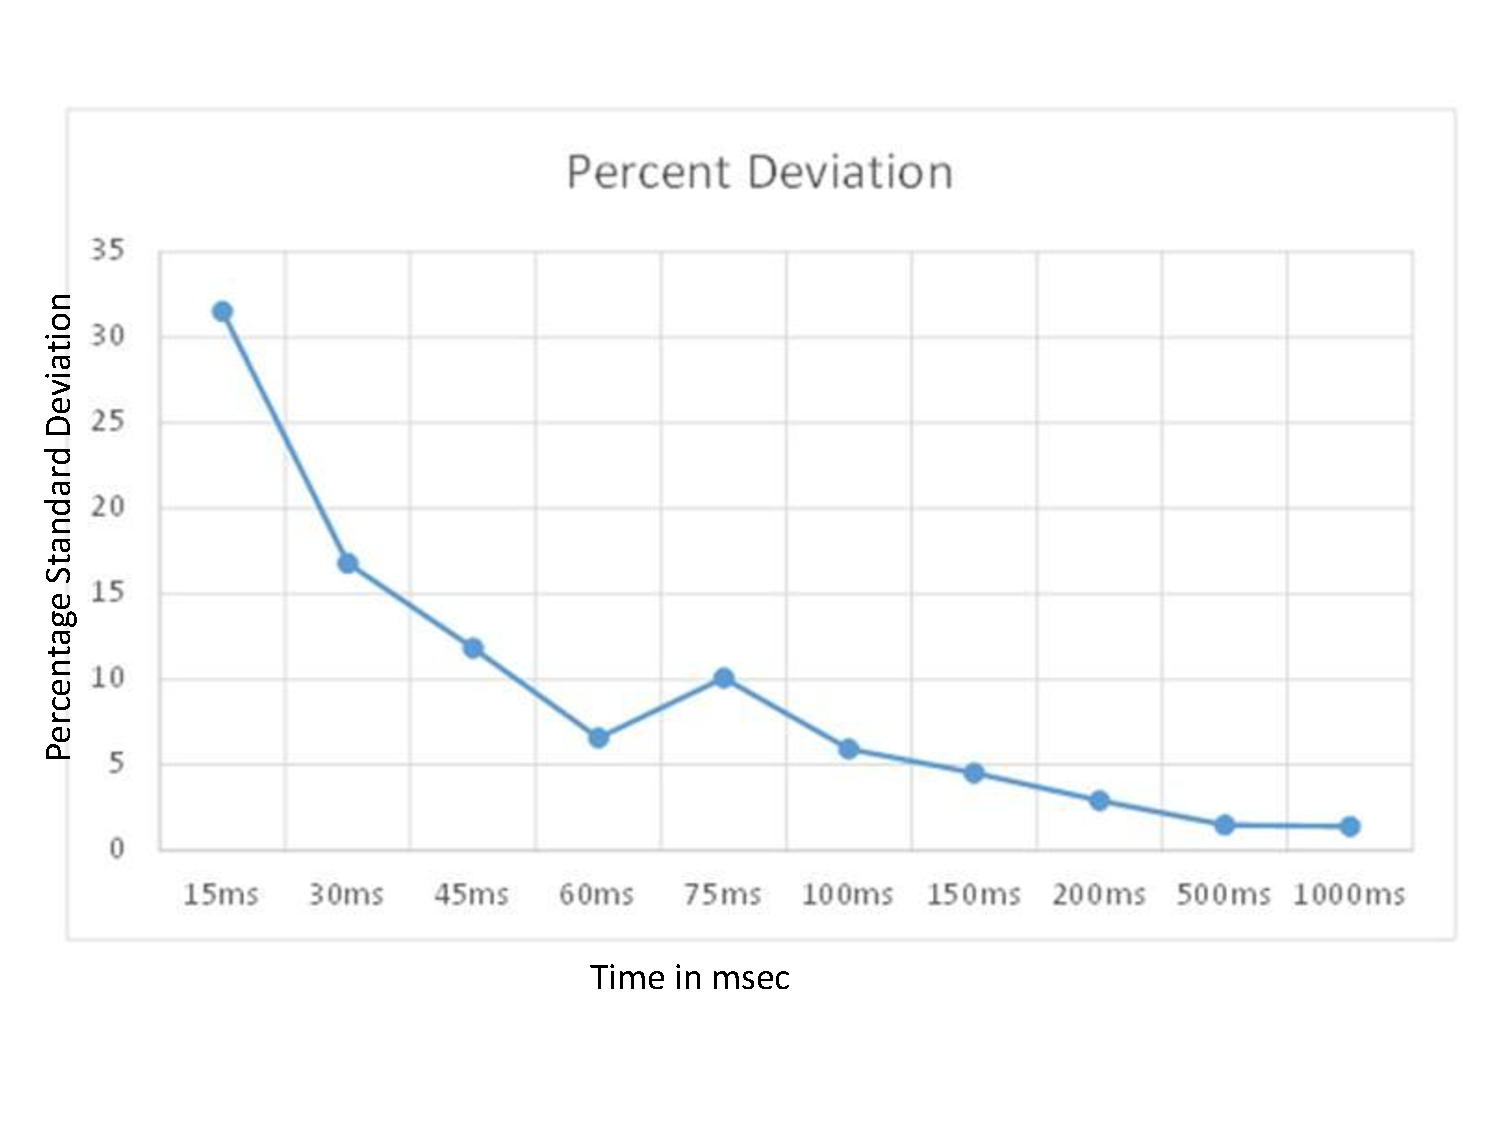
\includegraphics[width=\columnwidth, trim=60pt 20mm 0pt 8mm]{figures/variation}
\caption{Using too small a measurement interval for each period can cause a great deal of variance in the measured bandwidth}
\label{variation}
\vspace{-3mm}
\end{figure}

{\bf Discussion:} A value of $T$ between 60 - 100ms reduces standard deviation
of $SR$ to $5\%$.  Larger $T$ will lead to further reduction, but decrease is
small. 

\subsection{Bandwidth Ramp Up and Ramp Down}

{\bf Question:}  How fast does the algorithm allocate guaranteed bandwidth to a
customer ($T_{inc}$).  How fast does the algorithm reclaim bandwidth after a VM
reduces its bandwidth demands ($T_{dec}$?

{\bf Motivation:}  While the allocated badnwidth to VM ramps up to the minimum
guranteed bandwidth in 4 intervals, the VM may not be able to ramp up as
quickly, due to limiations of the TCP congestion control.

{\bf Experiment:}  The machine under test ("host machine") hosts 4 virtual
machines (VM) with the following minimum bandwidth guarantees: VM1: 100Mbps
(relative weight = 1), VM2: 100Mbps (relative weight = 1), VM3: 1Gbps (relative
weight: 10), VM4: 3Gbps (relative weight: 30) Each of the VMs sends traffic to
the other machine ("client machine") over the shared 10G external physical NIC.

Based on ideal fair queueing, one expects the following bandwidth allocations on the shared 10Gbps external NIC if all VMs are greedy and send as much as they are allowed to:
\begin{itemize}
\item VM1: 10000Mbps / (1+1+10+30) * 1 = 238Mbps
\item VM2: 10000Mbps / (1+1+10+30) * 1 = 238Mbps
\item VM3: 10000Mbps / (1+1+10+30) * 10 = 2.38Gbps
\item VM4: 10000Mbps / (1+1+10+30) * 30 = 7.14Gbps
\end{itemize}
 
And, should one of the VMs (e.g. VM4) stop using its bandwidth, one expects the residual bandwidth to be divided fairly (according to the subscribed weights) among the other VMs as followed:
\begin{itemize}
\item VM1: 10000Mbps / (1+1+10) * 1 = 833Mbps
\item VM2: 10000Mbps / (1+1+10) * 1 = 833Mbps
\item  VM3: 10000Mbps / (1+1+10) * 10 = 8.33Gbps  
\end{itemize}

The Windows Performance Monitor graph shown in Figure~\ref{fairsharing}  shows the transmit bandwidth for each VM, and the total transmit bandwidth of the physical NIC in for phases:

\begin{figure}[h]
\centering
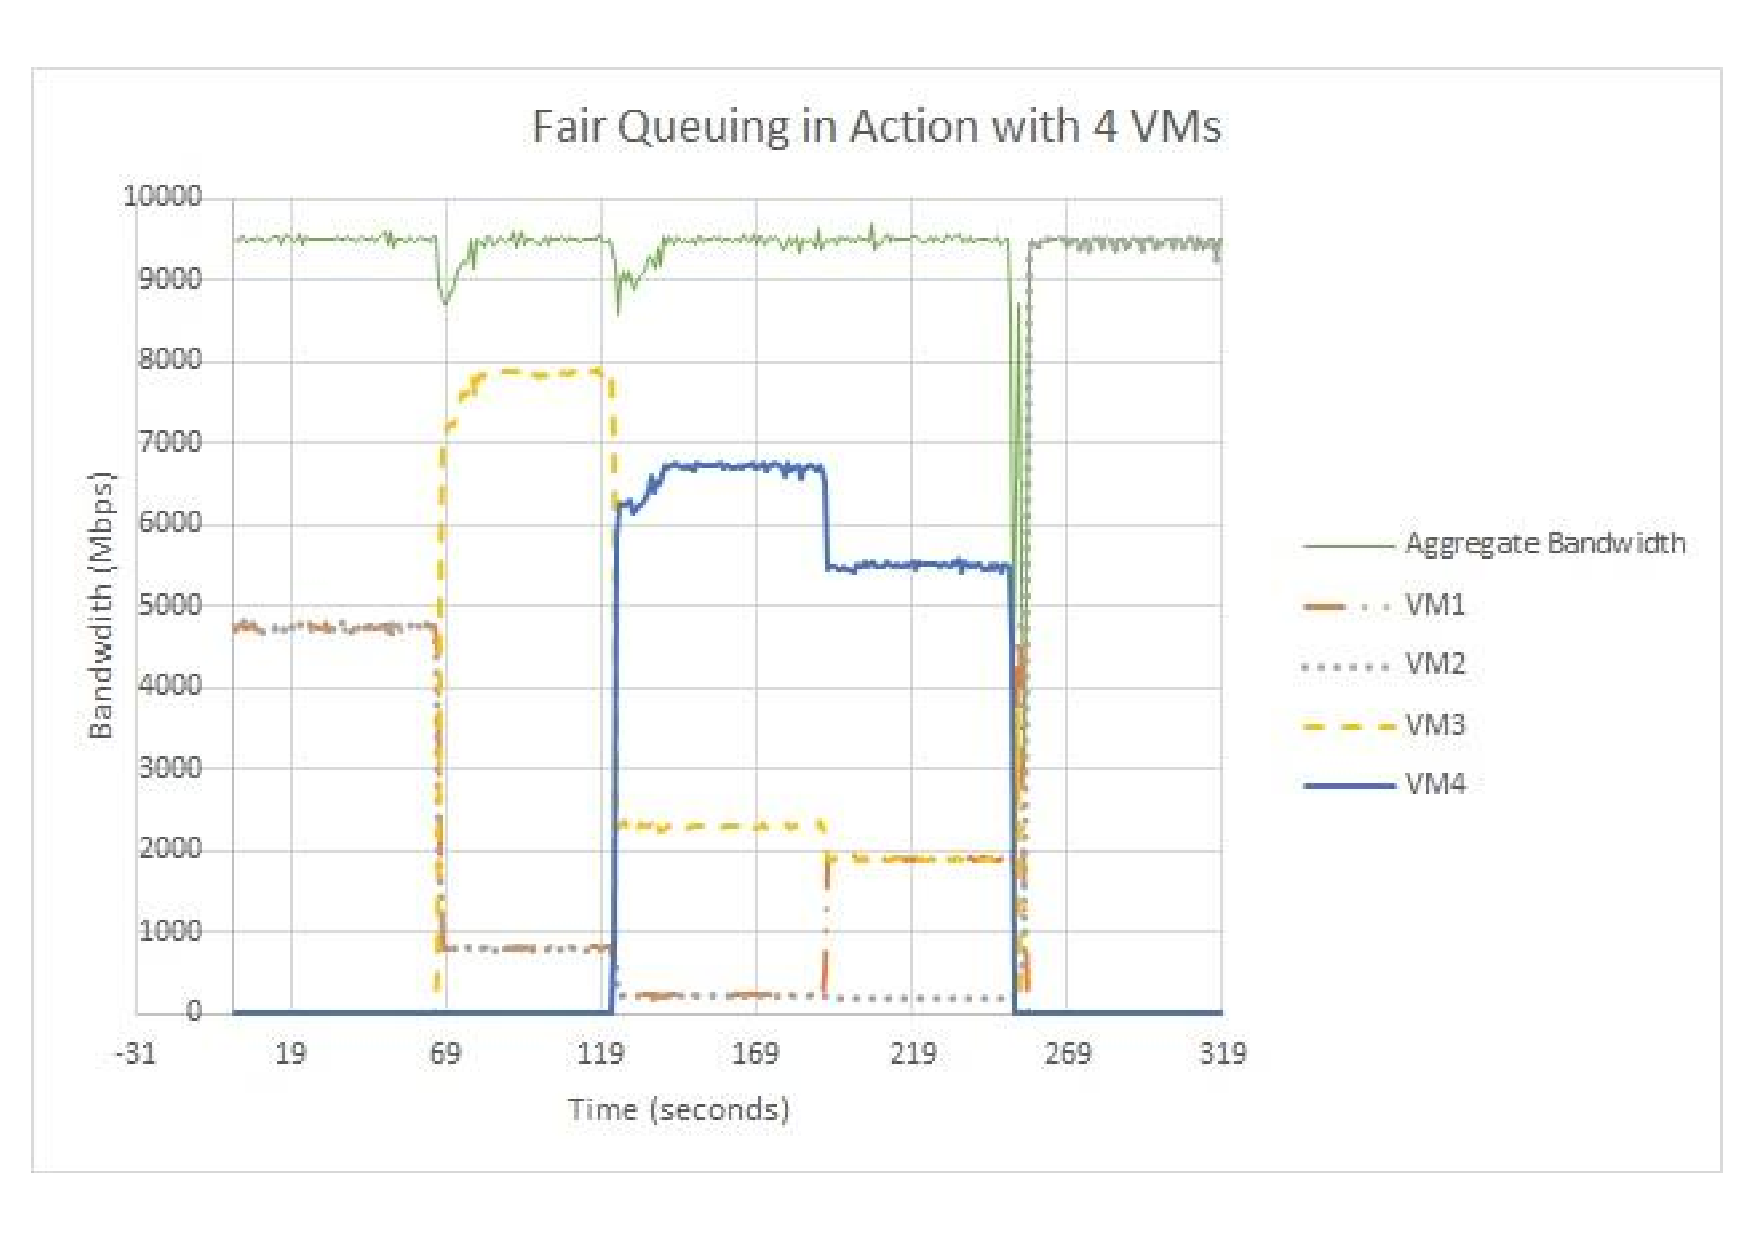
\includegraphics[width=\columnwidth,trim=60pt 20mm 0pt 8mm]{figures/fairsharing}
\caption{The ultimate test: can the algorithm distribute bandwidth fairly when VMs ramp up and ramp down.  The graph has 6 phases as shown below and involves 4 VMs}
\label{fairsharing}
\vspace{-3mm}
\end{figure}

{\bf Phase 1:}  VM1 and VM2 are sending as much data as they are allowed.

{\bf Phase 2:} VM3 joins VM1 and VM2.  VM1, VM2, and VM3 are sending as much data as they are allowed.

{\bf  Phase 3:} VM4 joins the other VMs. All VMs are sending as much data as they are allowed.

{\bf  Phase 4:} The IT administrator of the host machine changes the min bandwidth guarantee of VM1 from 100Mbps to 1Gbps.

{\bf Phase 5:} VM3 stops sending. VM1, VM2, and VM4 are sending as much data as they are allowed.

{\bf Phase 6:} VM1, VM3, and VM4 stop sending.  Only VM2 sends.

{\bf Discussion:} The dips in this graph are caused by the following behavior in
the algorithm: While VM3 and VM4 are ramping up, the algorithm detects that the
VMs requests for additional bandwidth in several consecutive iterations.
Therefore, in order to quickly provide the VMs their subscribed bandwidth, after
4 consecutive iterations of additional bandwidth requests, the algorithm
allocates the full fair share of bandwidth to the VM.  In this example, this
allocation of the full fair share is slightly more than the VM's actual
bandwidth need.  This dip represents a trade-off between how fast the algorithm
should grant a VM its fair share versus how cautious it should be in allocating
the VM bandwidth that it might not be ready to consume (and thus risk being
non-work conserving). In this scaenario, the algorithm strikes a good balance
between the two concerns. 

\subsection{Can we ramp up any faster?}

{\bf Question:}  Is the ramp up delay shown in Figure~\ref{fairsharing} for VM 4
at 69 seconds caused by our algorithm or it due to the VM itself (e.g., its TCP
behavior)?

{\bf Motivation:} The previous experiment suggests the algorithm may be too slow
in allocating bandwidth to a newly active VM.  

{\bf Experiment:} We measure bandwidth ramp up in two scenarios.  First, we
measure a  ``standalone'' scenario VM3 is the only VM transmitting (i.e. the link
was idle before VM3 started sending).  Second, we measure a  ``sharing'' scenario
in which the link was fully utilized before VM3 started sending. When VM3 starts
sending, MBFQ performs bandwidth allocation to give VM3 its fair share.

\begin{figure}[h]
\centering
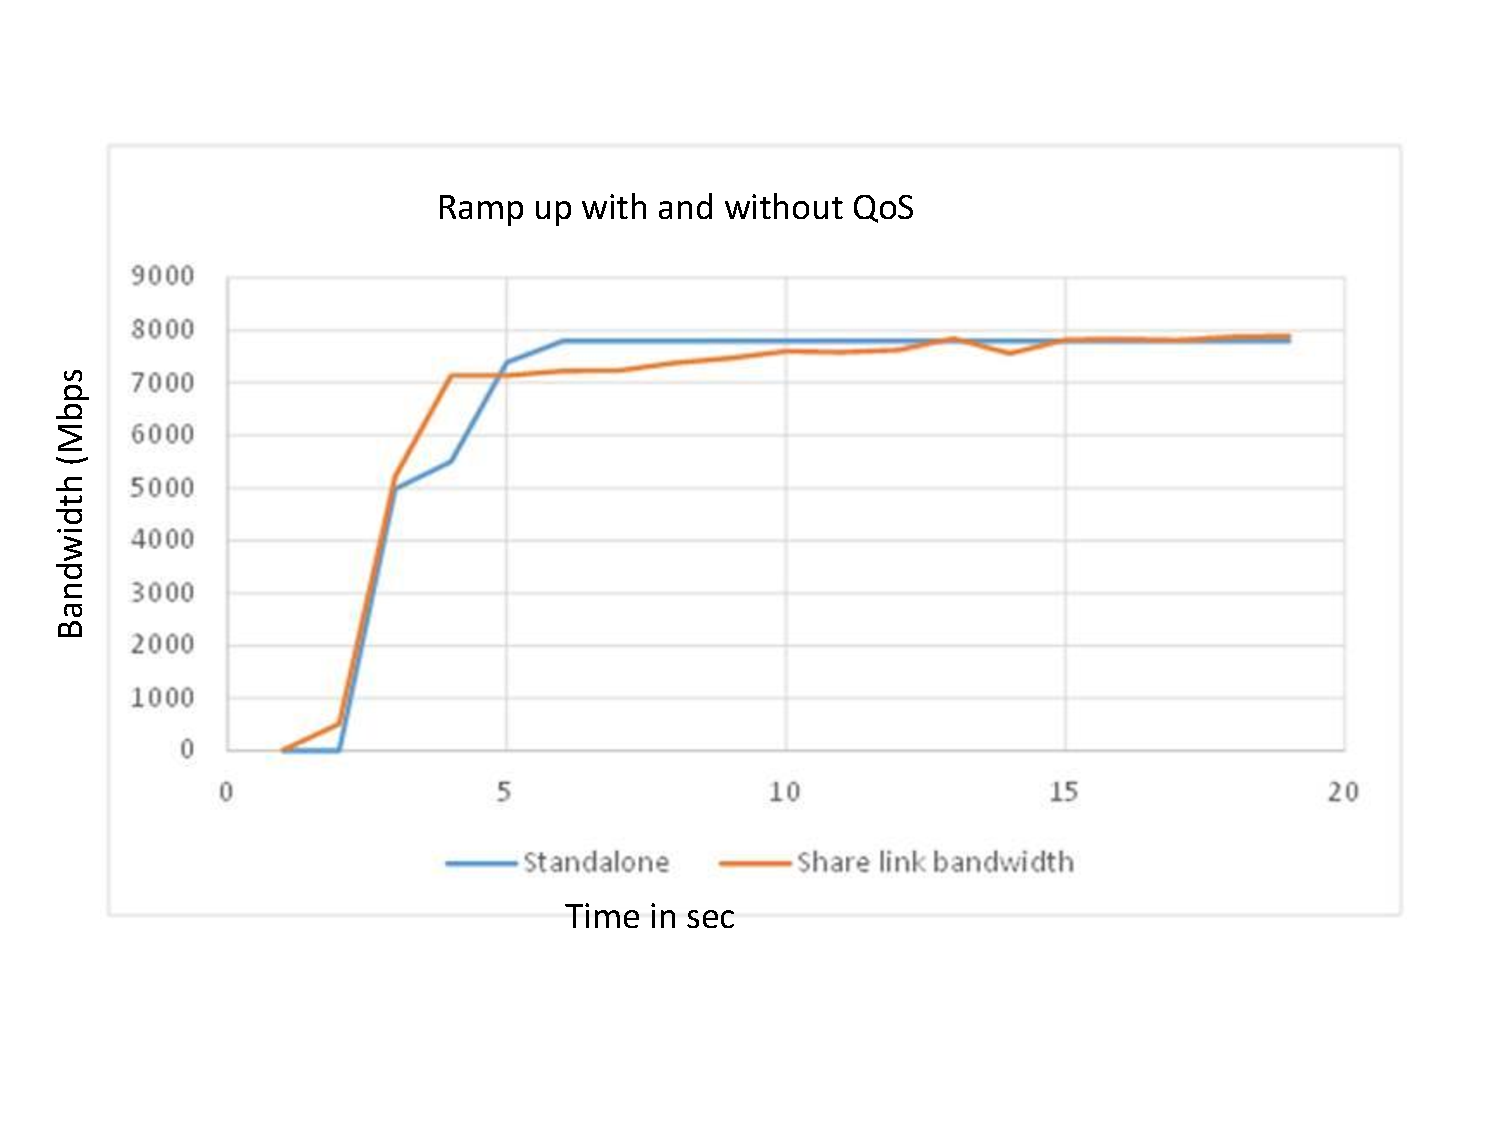
\includegraphics[width=\columnwidth,trim=60pt 40mm 0pt 8mm]{figures/rampupcomparison}
\caption{Comparing the ramp up speeds of TCP and MBFQ}
\label{rampupcomparison}
\vspace{-3mm}
\end{figure}

{\bf Discusion:} As seen in Figure~\ref{rampupcomparison}, it takes about the
same amount of time in both scenarios for VM3 to achieve most of its bandwidth
(up to 7Gbps). However, it takes an additional 15s for VM3 to reach its steady
state  in the "Share link bandwidth" scenario. However, in the sharing scenario,
the VM is transmitting on top of a NIC that is already fully utilized.
But in the standalone case, the VM is transmitting on top of an idle NIC. 

{\bf Conclusion:} It is probably not worthwhile trying to make MBFQ more agile
in ramping up faster because of inherent limitations to VM rampups due to
control algorithms such as TCP.

\subsection{How fast should we reclaim bandwidth}

{\bf Question:}  The faster we reclaim bandwidth the faster is $T_{dec}$, the
faster we redistrubute it other needy VMs who can use it.  How big should the
reclaim period $T$ be?

{\bf Motivation:} Figure~\ref{fairsharing} also shows a dip when VM1, VM3, VM4
stop sending.  In addition to the TCP ramp-up time of the app, the dip is also
partly due to another parameter in the algorithm where we configure the
algorithm to wait for 500ms before reclaiming residual bandwidth  Unfortunately,
this is a tradeoff.  The faster we reclaim, the more likely the algorithm is to
spuriously reclaim bandwidth from a paid customer VM which has short term
bursts.

{\bf Experiment:} : We have VM1, VM2, VM3 send CBR traffic. VM4 host a large
file that's being copied to a remote machine.  The file transfer application on
VM4 uses about 800Mbps, and the rest of the link bandwidth is distributed among
VM1, VM2, VM3.  We change the wait time parameter from No Wait (at every
macroscheduler iteration, bandwidth is immediately reclaimed if the VM is
sending less than 85\% of its allocated rate) to 1000ms wait (bandwidth is not
reclaimed unless the VM has been sending less than 85\% of its allocated rate in
the last 1000ms)
 
\begin{figure}[h]
\centering
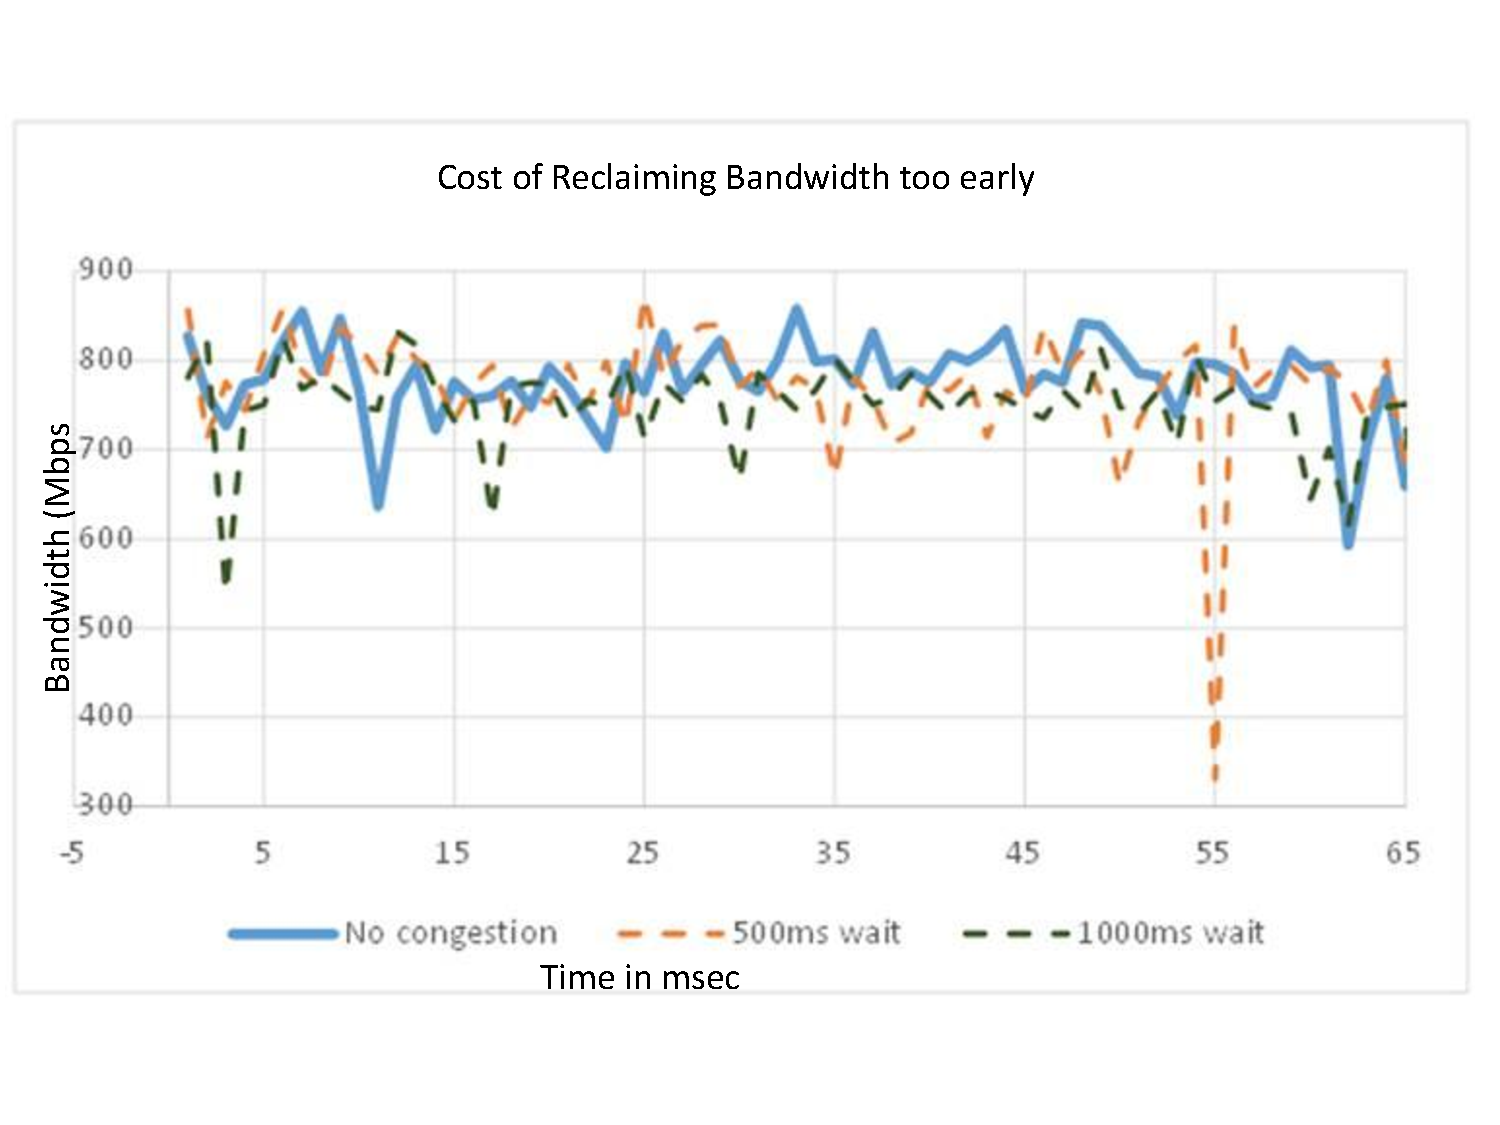
\includegraphics[width=\columnwidth,trim=60pt 20mm 0pt 8mm]{figures/rampdowntime1}
\caption{Bandwidth allocated to a bursty file transfer application with values of reclaim timer of 500 msec and 1000 msec}
\label{rampdowntime1}
\vspace{-3mm}
\end{figure}

Figure~\ref{rampdowntime1} shows that the bandwidth stays roughly the same with
MFQ and wihout MBFQ with a reclaim timer of 500 msec (in fact 1000 msec looks
even worse, but that could be an artifact).   On the other
hand,Figure~\ref{rampdowntime2} shows that with instantaneous reclaiming
(reclaim timer of 0) the bandwidth allocated to the VM is significantly affected
(by around 50\%) and its noticeable even at a reclaim timer of 200 msec.

\begin{figure}[h]
\centering
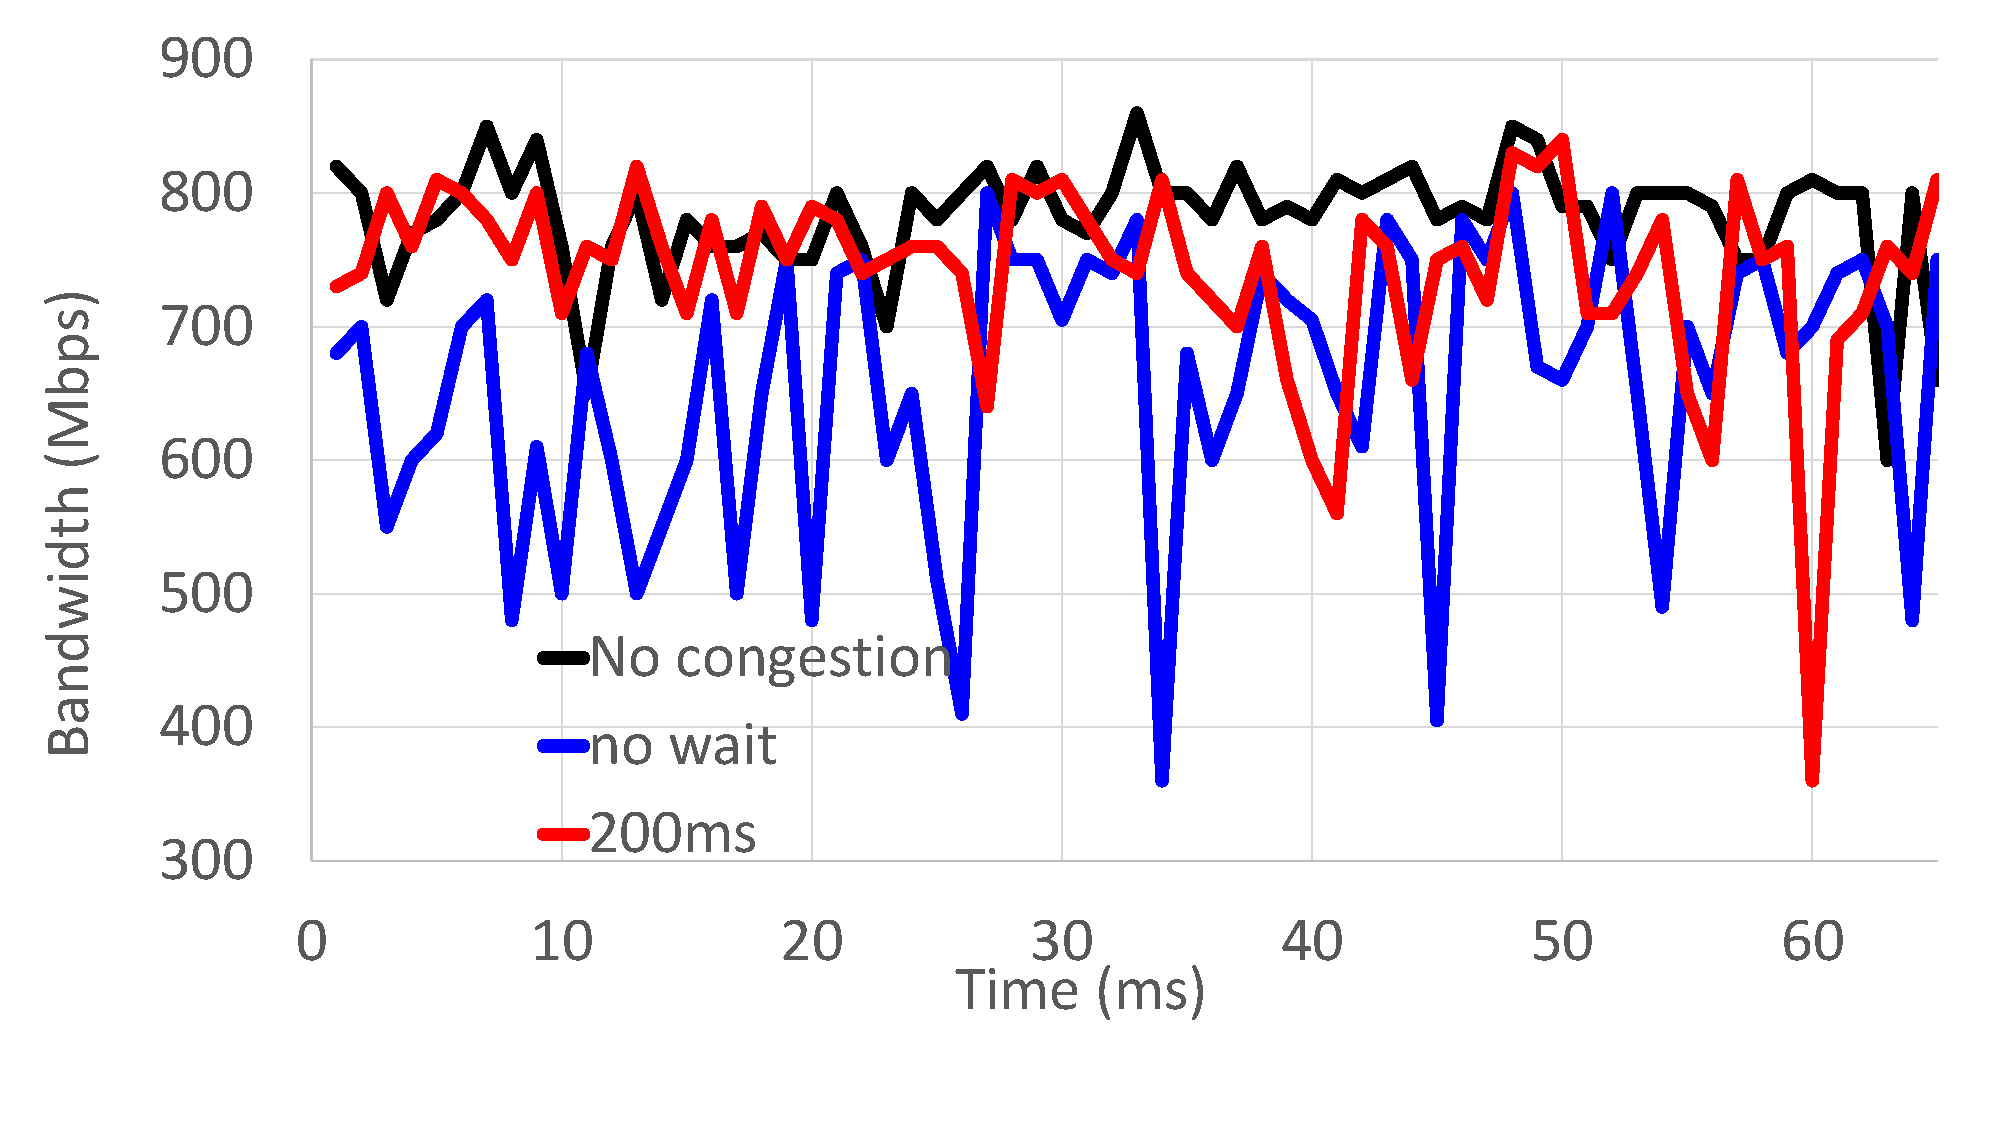
\includegraphics[width=\columnwidth,trim=60pt 20mm 0pt 8mm]{figures/rampdowntime2}
\caption{Bandwidth allocated to a bursty file transfer application with values of reclaim timer of 0 msec and 200 msec.  Notice the significant bandwidth loss due
to spurious reclamation}
\label{rampdowntime2}
\vspace{-3mm}
\end{figure}

{\bf Conclusion:}  A reclaim timer of around 500 msec seems like a good
compromise.  (Before our experimental evaluation, we had assumed that 1 sec
would be the right value). 
